\documentclass{article}
\usepackage{amsmath,amsfonts,amssymb,amscd}
\usepackage{tikz}\usetikzlibrary{fadings}
\usepackage[osf]{baskervillef}
\def\fsl{\mathfrak{sl}}
\def\fso{\mathfrak{so}}
\def\fg{\mathfrak{g}}
\def\fL{\mathfrak{L}}
\def\fA{\mathfrak{A}}
\def\fS{\mathfrak{S}}
\def\sA{\mathcal{A}}
\def\sR{\mathcal{R}}
\def\sD{\mathcal{D}}
\def\ZZ{\mathbb{Z}}
\def\NN{\mathbb{N}}
\def\RR{\mathbb{R}}
\def\CC{\mathbb{C}}
\def\TT{\mathbb{T}}
\def\XX{\mathcal{X}}
\DeclareMathOperator{\Der}{\mathrm{Der}}
\DeclareMathOperator{\End}{\mathrm{End}}
\DeclareMathOperator{\wt}{\mathrm{wt}}
\DeclareMathOperator{\gr}{\mathrm{gr}}
\DeclareMathOperator{\rk}{\mathrm{rk}}
\DeclareMathOperator{\pr}{\mathrm{pr}}
\def\p{\mathrm{p}}
\def\sm{\mathrm{sm}}
\title{Taming the infinite snake}
\author{JG}
\newtheorem{lem}{Lemma}
\newtheorem{prop}{Proposition}
\begin{document}
\sloppy\maketitle

\section{Introduction}
\label{sec:intro}
\subsection{Overview}
This paper is devoted to a simple mechanical
system with remarkable mathematical properties.
The \emph{infinite snake} is a sequence of 
identical rigid segments, connected by
planar rotating joints; each segment is
equipped with a wheel attached in the middle,
and the wheels roll 
on a plane with no slipping
or skidding (\textbf{figure}). The latter condition 
imposes non-holonomic constraints on the system's kinematics.
Our central observation is that
this kinematics realises, in a formal sense, the positive
subalgebra of the 
\emph{twisted loop algebra} of $\fsl_2(\RR)$. 

The statement is easy to formulate. Reducing by obvious translational
symmetry, the snake's configuration space may be identified with an
infinite torus $\TT^\infty = \varinjlim_{n\to\infty} \TT^n$, parameterising
the orientations of subsequent segments.
It is an exercise in imagination to see that the snake `follows its head':
that is, the motion of the entire system is determined by the initial configuration,
and the curve traced by the free endpoint of the first segment (\textbf{figure}). 
In particular, at every given configuration one may consider the two motions characterised
by the `head' moving along either axis of a fixed Cartesian coordinate system on the plane.
Infinitesimally, these correspond to a pair of vector fields $X$, $Y$ on $\TT^\infty$.
The Lie algebra $\fS$ generated by these two will be our main object of study.

Now, the twisted loop algebra referred to above is
$$
L_\theta\fsl_2(\RR) = \{ u(t)\ |\ u(-t)=-u(t)^T \} \subset \fsl_2(\RR)[t,t^{-1}] = L\fsl_2(\RR)
$$
where $\theta$ refers to the Cartan involution $u \mapsto -u^T$ on $\fsl_2(\RR)$.
The latter leads to a decomposition $\fsl_2(\RR) = \fso_2(\RR) \oplus \RR^2$ into eigenspaces,
and we may describe $L_\theta\fsl_2(\RR)$ as a $\ZZ$-graded Lie algebra with copies of 
$\fso_2(\RR)\simeq\RR$ in even degrees, and of $\RR^2$ in odd degrees.
The positive subalgebra $L_\theta^+\fsl_2(\RR)$ is the sum of positively graded subspaces:
$$
L_\theta^+\fsl_2(\RR) = L_\theta\fsl_2(\RR) \cap t \fsl_2(\RR)[t].
$$
Our main result then states that there is an orthogonal
basis $x,y\in\RR^2$ such that the map $X\mapsto tx$, $Y\mapsto ty$
extends to an \emph{isomorphism} of Lie algebras
$$\fS \simeq L_\theta^+\fsl_2(\RR). $$

The proof of this isomorphism is fairly non-trivial. We will exploit certain symmetries
of the snake to express the serpentine Lie algebra $\fS$ in a more abstract fashion,
and proceed with a rather explicit computation. 

\subsection{Motivaiton}
Truncating the snake's tail after finitely many segments
produces a finite system inheriting some properties of 
its infinite form. 
These finite snakes are interesting as actual
robotic systems effectuated by bending the joints (the wheels are passive). 
M. Ishikawa studied the three-segment snake in \textbf{[refs]},
coming up with a beautiful control-theoretic application of
principal connections and the Ambrose-Singer theorem. He also worked on other robots based on
effectuated joints and rigid segments with passive wheels, such as
the `trident snake' \textbf{[ref]}.

Around 2014, partly inspired by Ishikawa's work, P. Nurowski proposed 
a systematic study of the geometries associated with all snake-like systems: 
that is, planar graphs with edges corrseponding to rigid segments of fixed
length, some equipped with wheels at a fixed location along the edge. 
Given the configuration space $M$ of such a `generalised snake', 
the condition of no skidding and no skipping imposed on each wheel
gives rise to a constraint distribution $\sD \subset TM$ (one may 
exclude some degenerate configurations, thus restricting $M$ to an 
open subset over which $\sD$ has constant rank). Then one studies
the flag $\sD^\bullet$ defined inductively by $\sD^1 = \sD$,
$\sD^{i+1}=[\sD,\sD^i]$, so that $\sD^{i}$
is spanned by $i$-fold iterated Lie brackets of sections of $\sD$
(one may further shrink $M$ to an open subset over which
the $\sD^i$ have constant rank). Assuming the snake system is \emph{controllable},
i.e. that $\bigcup \sD^i=TM$, we have that $\sD^\bullet$
forms an exhaustive filtration of $TM$. One then studies the associated graded
bundle $\gr TM$, of rank equal to the dimension of $M$. By construction, the Lie
bracket of vector fields induces a Lie algebra structure in each fibre of $\gr TM$.
The graded nilpotent Lie algebra $\gr T_x M$ is called the \emph{symbol} of $\sD$ at $x$, and forms
an important local algebraic invariant of the non-holonomic distribution $\sD$.

Up to the data of segment lengths and wheel positions, these generalised snakes
are of combinatorial nature; in particular, as graphs, they admit an inductive
description, where a system is built by attaching edges (with or without wheels)
one at a time. Working in Nurowski's project, I considered the possibility of exploiting
such inductive descriptions to compute the symbol at a general configuration.
A more modest goal would be to predict the snake's \emph{growth vector}: that is
the sequence $(\rk\sD^i)_{i>0}$; equivalently, we might consider
$(\rk \gr_iTM)_{i>0}$, i.e. 
the sequence of dimensions
of graded homogeneous subspaces of the \emph{symbol} $\gr T_x M$ at a general point.
The former is the cumulative sum of the latter, which we may thus call the
\emph{growth rate vector}.

I've thus quickly arrived at the problem of computing the growth vector of
the $n$-segment snake -- the result of iteratively attaching a wheeled edge  
to a free endpoint of the system. An explicit calculation with help of computer
algebra gives the following results:
\begin{center}\fbox{
\begin{tabular}{c|l||c|l||c|l}
        $n$ & growth rate&
        $n$ & growth rate&
        $n$ & growth rate\\
        \hline
        1 & 2 1 & 
        4 & 2 1 2 1 &
        7 & 2 1 2 1 2 1
        \\
        2 & 2 1 1 &
        5 & 2 1 2 1 1 &
        8 & 2 1 2 1 2 1 1 
        \\
        3 & 2 1 2 &
        6 & 2 1 2 1 2 &
        9 & 2 1 2 1 2 1 2
\end{tabular}
}\end{center}
A clear pattern emerges -- how does one explain it?
Up to some irregularity at the `tail', the growth rate
vector appears to be a string of 2 1 2 1 2 1 2 \dots,
suggesting that the results for finite snakes may be the shadow
of a simpler situation in the limit $n\to\infty$. 

There are some remarkable features of the snake to be pointed out in this context.
First, the symbol (at a general point) of each of the $n$-segment
snakes appears to have \emph{width} 2 (that is the bound on
the dimensions of homogeneous graded components). This is
very far from the generic situation, and puts the sequence
of snakes in a similar category as the much studied sequence
of \emph{trailers}, systems with growth rate 2 1 1 1 \dots (indeed, deforming the $n$-segment snake
by varying the position of the wheels, and then degerating by moving each wheel to
an endpoint of its segment, one ends up with an $n$-segment trailer). 
Second, in the infinite snake, the symbol of $\sD$ actually coincides with
the Lie algebra generated by the vector fields $X, Y$ spanning $\sD$ (that doesn't
happen for finite snakes, where -- unlike the symbol -- the algebra generated
by the two vector fields isn't nilpotent).
All these points will be taken up more formally in Section \ref{sec:further}.

\subsection{Approach}
It is easy to \emph{conjecture} the isomorphism $\fS \simeq L^+_\theta\fsl_2(\RR)$
based on explicit computation,\footnote{I've presented the conjecture and some of its
ramifications at a 2015 Bedlewo workshop on Nonlinear Control.}
but actually proving it requires tackling two infinities: the depth of iterated Lie brackets,
and the length of the snake.
The former involves straightforward induction on bracket depth.
The latter will be approached through a less obvious \emph{corecursion}.

The corecursion is related
to a particular `symmetry' of the infinite snake that becomes broken
in its finite sub-snakes:
namely, the tail, that is the
snake minus its initial segment,
is still an infinite snake.\footnote{Of course cutting the snake's head off
is not invertible, whence one should rather speak of a \emph{pseudo-}symmetry.}
This gives rise to a `shift operation', passing from the original snake to its
tail. We shall furhter twist it using the obvious Euclidean symmetry of the system
(since we have already reduced the configuration space by translations,
we are left with rotations and reflections). 

So far, we haven't really specified the parameterisation identifying the infinite snake's
reduced configuration space with $\TT^\infty$. Let us temporarily denote the
former more abstractly as $M$. Now, identify the configuration space
of the one-segment snake with $\TT$, parameterised by an angle coordinate $\varphi$
such that $\varphi=0$ corresponds to the segment being aligned with the first
Cartesian axis (the one associated with $X$). Let $$ \TT \xleftarrow{\pi_h} M \xrightarrow{\pi_t} M $$
be the projections sending the configuration $m$ of an infinite snake 
to, respectively, the configuration of its initial segment, $\pi_h(m)$,
and the configuration
of its tail \emph{as} an infinite snake, $\pi_t(m)$.
Now, let $$ S, R_\vartheta : M \to M $$
denote the symmetries induced by, respectively,
reflection about the first Cartesian axis, and
rotation by $\vartheta \in \TT$. Define
$$ R : \TT \times M \to M,\quad R(\vartheta, m) = R_\vartheta(m) $$ 
and 
consider the \emph{invertible} map
$$
\Phi : M \xrightarrow{\langle \pi_h,\pi_t\rangle} \TT \times M
\xrightarrow{\langle \pr_1, S \circ R\rangle} \TT \times M.
$$
That is, $\Phi$ sends a configuration of the infinite snake
to the pair: the configuration of its initial segment, and
the configuration of its tail, but in a coordinate system
whose first axis is parallel to the initial segment, and
whose orientation is reflected.

Iterating the map $\Phi$ produces a sequence of invertible maps
$\Phi^{(n)} : M \to \TT^n \times M$ and, in the limit,
an identification 
$$\pr_1 \circ \Phi^{(\infty)} : M \longrightarrow \TT^\infty = \varprojlim_{n\to\infty} \TT^n.$$
With standard angle coordinates $(\varphi_1,\varphi_2,\dots)$ on $\TT^\infty$,
the above identification corresponds to parameterising the infinite snake
as in Figure~\ref{fig:param}.

\begin{figure}\begin{center}
        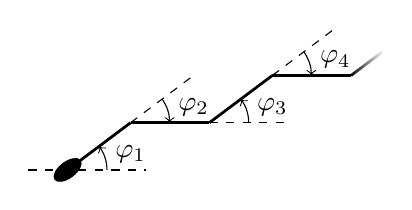
\begin{tikzpicture}
                \draw[dashed] (-0.5,0) -- (1.0,0);
                \draw[line width=1] (0,0) -- (0.8,0.6);
                \draw[dashed] (0.8,0.6) -- (1.6,1.2); 
                \draw[line width=1] (0.8,0.6) -- (1.8,0.6); 
                \draw[dashed] (1.8,0.6) -- (2.8,0.6);
                \draw[line width=1] (1.8,0.6) -- (2.6,1.2); 
                \draw[dashed] (2.6,1.2) -- (3.4,1.8); 
                \draw[line width=1] (2.6,1.2) -- (3.6,1.2); 
                \draw[line width=1,path fading=east] (3.6,1.2) -- (4.0,1.5);
                \draw[->] (0.5,0) arc (0:36:0.5); \node at (0.8,0.2) { $\varphi_1$ };
                \draw[->] (2.3,0.6) arc (0:36:0.5); \node at (2.6,0.8) { $\varphi_3$ };
                \draw[->] (1.2,0.9) arc (36:0:0.5); \node at (1.6,0.8) { $\varphi_2$ };
                \draw[->] (3.0,1.5) arc (36:0:0.5); \node at (3.4,1.4) { $\varphi_4$ };
                \draw[rotate=37,fill] (0,0) ellipse (0.2 and 0.1);        
        \end{tikzpicture}\end{center}
        \caption{Parameterisation defined by $\pr_1\circ\Phi^{\infty} : M \to \TT^\infty$.
        \label{fig:param}}
\end{figure}

It turns out that the vector fields $X$, $Y$ admit a convenient corecursive
description with respect to $\Phi$. Let $\XX^\p(M)$ denote the space of
smooth projectable vector fields on $M$ (that is an inverse limit of 
spaces of smooth projectable vector fields on the configuration spaces of finite sub-snakes),
and let
$$ \XX(\TT) \xrightarrow{\iota} \XX^\p(M) \xleftarrow{\Sigma} \XX^\p(M) $$
be the maps induced by $\Phi^{-1} :  \TT\times M \to M$. Note that these in turn induce
an isomorphism\footnote{For simplicity, at this stage we use
smooth functions, whence the need for a completed tensor product.
In Sec.~\ref{sec:algebra} we will actually 
work with Laurent polynomials on complex tori.}
$$
\XX(\TT) \oplus C^\infty(\TT) \widehat\otimes \XX^p(M) \to \XX^\p(M),
\quad
(v, f \otimes V) \mapsto \iota v + (\pi_h^* f)\cdot \Sigma V.
$$
It will be most convenient to complexify and consider
$Z = X+iY \in \CC\otimes\XX^\p(M)$.
Then, we find the following corecursive formula (see Section~\ref{sec:basic}):
$$
Z = -e^{i\varphi} \left( 
        \Sigma Z + i(\Sigma-1)\iota\partial_\varphi
\right)$$
where we view $\varphi$ as a function on $M$ via $\pi_h^*$.
Since the operator $1+e^{i\varphi}\Sigma$ 
is invertible on $\XX^\p(M)$, the above does indeed determine $Z$. A
conjugate formula holds for $\overline Z = X - iY$, and it is not unreasonable
to expect such recursive formulas for their iterated Lie brackets.
These are derived in Section \ref{sec:algebra}. In particular,
we find that the Lie algebra $\fS_\CC$ generated by $Z, \overline Z$
(a complexification of $\fS$) is isomorphic to $L_\theta^+\fsl_2(\CC)$.
Then, passing to real forms we conclude with $\fS\simeq L_\theta^+\fsl_2(\RR)$.


\subsection{Consequences}

\subsection{Acknowledgements}


\section{Basic construction}
\label{sec:basic}
\subsection{A single segment}

\subsection{Growing the tail}

\subsection{Abstracting the symmetry}

\section{Serpentine Lie algebra}
\label{sec:algebra}
\section{Further discussion}
\label{sec:further}
\end{document}
